\documentclass[a4paper]{article}
%\setbeameroption{show notes on second screen=right} % Both
% Theme choice:
\usepackage{geometry}
\geometry{
	a4paper,
	total={170mm,257mm},
	left=20mm,
	top=20mm,
}
\usepackage{tikz-feynman}
\usepackage{animate}
\usepackage{amsmath}
\usepackage{cancel}
\usepackage{multicol}
\usepackage{physics}
\usepackage{graphicx}
\usepackage{amsfonts}
\usepackage{caption}
\usepackage{wrapfig}
\usepackage{pgfplots}
\usepackage{subfigure}
\usepackage{listings}
\pgfplotsset{compat=1.15}
\captionsetup{singlelinecheck=false}
\usepackage[backend=bibtex,bibencoding=utf8,doi=false,isbn=false,url=false,eprint=false,indexing=false,style=authoryear]{biblatex}
\addbibresource{library}
\AtEveryBibitem{%
	\clearname{translator}%
	\clearlist{publisher}%
	\clearfield{pagetotal}%
}
\usepackage{MnSymbol,wasysym}
\usepackage[toc,page]{appendix}
\usetikzlibrary{snakes}
\usetikzlibrary{shapes.geometric, calc}
\author{Vo Chau Duc Phuong}
% Title page details: 
\title{Simulation of Liquid Argon}
\begin{document}
	\maketitle
\tableofcontents
\section{Introduction}
\quad Using the FORTRAN, I simulate the liquid Argon in the Lennard-Jones potential between the particles. The input value into the code will be these parameters and variables:\\
\rule{\textwidth}{1pt}
{\small
 \begin{lstlisting}
integer :: n = 864, bc = 1, tr = 0 !bc: periodic boundary, tr: poor-mans algorithm
real, allocatable :: dens(:,:,:)
!crucial parameters
real, parameter :: T = 94.4, kb= 1.380649*10.**(-16.)
real, parameter :: m = 39.95*1.67*10.**(-24), sigma = 3.4*10**(-8.)
real, parameter :: ep = 120.*kb, rc = 2.25, L = 10.229, halfL = 10.229/2.
!time parameters
integer :: nt, ntrelax
real, parameter :: tmin = 0.0, tmax = 100.0, trelax = 10.0 !in ps
real ::  dt = 0.01  !ps
\end{lstlisting}}
\rule{\textwidth}{1pt}\null\vspace{0.5cm}
\normalsize\null
\quad The first line is specify the number of particles, use the parameter and poor-mans thermal-stat or not. (in this case, no thermal-stats).\\\null
\quad Second line is the define of the density matrix, contains the position and velocity of all particles.\\\null
\quad Crucial parameter will be in the unit of cgs. The time parameters as shown.\\
\rule{\textwidth}{1pt}
{\small
\begin{lstlisting}
subroutine Initial()
implicit none
integer :: i, j, k, p
real :: spacing, v_stddev, rand1, rand2, Tp, E
allocate(dens(n,3,2))
ntrelax = int(trelax/dt); nt = int((tmax - tmin)/dt)
dt = dt*1.0e-12*(ep/m)**0.5*1./sigma
! Initialize densitions randomly within the box
spacing = L / (int(n**(1.0/3.0)) + 1) ! Adjust spacing to avoid boundary
p = 0
do i = 0, int(n**(1.0/3.0))
do j = 0, int(n**(1.0/3.0))
do k = 0, int(n**(1.0/3.0))
p = p + 1
if (p > n) exit
dens(p,1,1) = i * spacing
dens(p,2,1) = j * spacing
dens(p,3,1) = k * spacing
end do
if (p > n) exit
end do
if (p > n) exit
end do
v_stddev = sqrt(kb * T / m)
do i = 1, n
do j = 1, 3
call random_number(rand1); call random_number(rand2)
dens(i,j,2) = v_stddev * sqrt(-2.0 * log(rand1)) &
* cos(2.0 * 3.14159265359 * rand2)
end do
end do
do i = 1, 3
dens(:,i,2) = dens(:,i,2) - sum(dens(:,i,2))/n
end do
Tp = sum(dens(:,:,2)**2.) * m / (3.0 * n * kb)
dens(:,:,2) = dens(:,:,2) * sqrt(T / Tp)
dens(:,:,2) = dens(:,:,2) / (ep/m)**0.5 ! Convert to dimensionless units
end subroutine
\end{lstlisting}}
\rule{\textwidth}{1pt}\\\null
\quad First, I generate the position of the particles in a lattice to avoid the very strong at the near interaction of Leornard-Johnes potential and also generate the velocity in each direction arcording the Boltzmann distribution using random-number generator.
\begin{figure}[h]
\begin{center}
	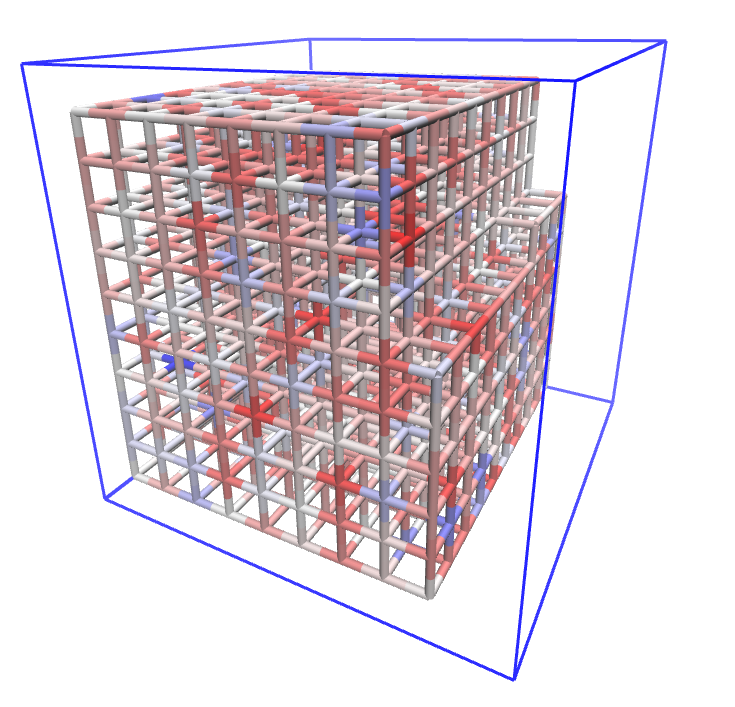
\includegraphics[width = 0.5\linewidth]{Images/Lattice.png}
\caption{Initial position of atoms and their colored according to their initial velocity}
\end{center}
Then, using the do loop, delete the net-momentum velocity. After all, scale every thing to our desire temperature using the relation: \(v \sim \sqrt{T}\) and converge to the dimensionless unit (which position is already in). According to the paper, the unit of length is \(\sigma\), the unit of velocity is \(\sqrt{\epsilon/m}\) and the unit of time is \(10^{-12}*(\epsilon/m)^{1/2}(1/\sigma)\) (the line with \(dt = dt...\)) to match which the rest.
\end{figure}
\section{Method}
\section{Results and Discussion}
\end{document}